\chapter{测试系统的特性}
\label{hw:systems}

\noindent 本章对应《课后作业-CH3》的全部4题。数值答案以静态灵敏度标定后的输出为准，取归一化静态增益 $K=1$；相角差统一定义为“输出相位减输入相位”。知识说明中保留一般静态灵敏度 $K>0$；实际输出幅值需再乘 $K$，归一化幅值误差与相位结论不变。

\section{第1题：双频信号通过一阶装置}
\label{hw:3-1}
\begin{hwquestion}
求周期信号 $x(t)=0.5\cos(10t)+0.2\cos(100t-45^\circ)$ 通过传递函数
$H(s)=1/(0.005s+1)$ 的装置后得到的稳态响应。要求根据线性叠加特性和一阶系统动态特性计算，并分析不同频率的幅值、相位变化规律。
\end{hwquestion}

\subsection*{答案与解析}
由 $\tau=0.005\,\mathrm{s}$ 得
\[
H(\iu\omega)=\frac{1}{1+\iu0.005\omega},\qquad
A(\omega)=\frac{1}{\sqrt{1+(0.005\omega)^2}},\qquad
\phi(\omega)=-\arctan(0.005\omega).
\]
稳定线性时不变系统对每个正弦分量分别作“幅值乘 $A$、原相位加 $\phi$”的变换。两个分量的角频率为 $10$ 与 $100\,\mathrm{rad/s}$，于是
\begin{align*}
A_1&=(1+0.05^2)^{-1/2}=0.998752,
&\phi_1&=-\arctan0.05=-2.8624^\circ,\\
A_2&=(1+0.5^2)^{-1/2}=0.894427,
&\phi_2&=-\arctan0.5=-26.5651^\circ.
\end{align*}
因此 $y_1(t)=0.499376\cos(10t-2.8624^\circ)$，
$y_2(t)=0.178885\cos(100t-45^\circ-26.5651^\circ)$。叠加得
\[
\boxed{\begin{aligned}
y_{\mathrm{ss}}(t)\approx{}&0.499376\cos(10t-2.8624^\circ)\\
&+0.178885\cos(100t-71.5651^\circ).
\end{aligned}}
\]
相位中的度数是常相位的标注；用计算程序求值时须转为弧度。

\begin{center}
\small
\begin{tabular}{@{}ccccc@{}}
\toprule
$\omega/(\mathrm{rad/s})$ & 输入幅值 & 输出幅值 & 幅值衰减 & 系统相角差\\
\midrule
$10$ & $0.5$ & $0.499376$ & $0.1248\%$ & $-2.8624^\circ$\\
$100$ & $0.2$ & $0.178885$ & $10.5573\%$ & $-26.5651^\circ$\\
\bottomrule
\end{tabular}
\end{center}
频率升高时，一阶装置的幅值比单调降低，相位由 $0$ 向 $-90^\circ$ 滞后；输出各分量仍与各自输入同频。高频项受到更强衰减和更大相位滞后，故叠加后的波形发生变化。

\begin{focusbox}{知识主线}
把装置看成稳定线性时不变系统：由微分方程建立 $H(s)$，令 $s=\iu\omega$ 得到正弦稳态的幅值比与相位差，最后逐频叠加。下文依次解释这些步骤的依据，以及为什么同频输出仍可能改变多频波形。
\end{focusbox}

\subsection*{本题知识点与公式}
\label{kn:3-1}
\noindent\textbf{已学前置：}第\ref{kn:2-2}节的复数频谱、幅值与相位，第\ref{kn:2-4}节的卷积与时频域联系。
\textbf{本题新增：}系统的线性与时不变性、传递函数和初值条件、冲激响应、一阶模型、相量稳态法、稳态与暂态及不失真测量。

\subsubsection*{1. 为什么可以分开计算两项：线性、时不变与零状态}
用 $\mathcal T$ 表示装置对输入的作用。若在\textbf{零初始状态}下 $x_1\mapsto y_1$、$x_2\mapsto y_2$，线性要求对任意常数 $a,b$ 都有
\[
\mathcal T\{ax_1+bx_2\}=a\mathcal T\{x_1\}+b\mathcal T\{x_2\}.
\]
其中 $a\mathcal T\{x_1\}$ 是比例性，两种输入响应相加是叠加性。因此本题可以分别求两项的响应再相加。零状态意味着储能元件没有额外初始能量，例如电容初始电压或机械质量块初始位移、速度为零。存在初始能量时，还要单独加入它引起的零输入响应，不能把该响应重复加入每一项。

时不变性则要求输入整体延后 $t_0$，输出也仅延后相同时间：
\[
\mathcal T\{x(t-t_0)\}=y(t-t_0).
\]
常系数线性微分方程在相应的固定工作条件下给出典型的线性时不变（LTI）模型。线性与时不变是两项要求；调制环节 $y(t)=x(t)\cos\omega_ct$ 对输入线性，却因系数随时间变化而不是时不变系统，会搬移频率。\textbf{本题逐频保持原频率的结论依赖稳定LTI模型，而不只是“线性”二字。}实际装置发生饱和、明显迟滞或参数随工况变化时，应重新检查这一模型是否适用。

\subsubsection*{2. 从微分方程到传递函数：$H(s)$ 包含什么信息}
若输入 $x(t)$、输出 $y(t)$ 满足
\[
a_1\dot y(t)+a_0y(t)=b_0x(t),
\]
在 $a_0\ne0$ 时除以 $a_0$，令 $\tau=a_1/a_0$、$K=b_0/a_0$，就得到一阶标准模型
\[
\boxed{\tau\dot y+y=Kx},\qquad \tau>0.
\]
例如电阻、电容构成的低通电路满足 $RC\dot u_C+u_C=u_{\mathrm{in}}$，故 $\tau=RC$、$K=1$。机械、热学等装置的一个主要惯性过程也可能在限定工作范围内近似成相同形式；“一阶”指最高时间导数为一阶，并非指输入只有一个频率。

引入拉普拉斯变换 $X(s)=\int_{0^-}^{\infty}x(t)e^{-st}\diff t$，其中 $s=\sigma+\iu\omega$ 为复频率。用
$\mathcal L\{\dot y\}=sY(s)-y(0^-)$ 得
\[
(\tau s+1)Y(s)=KX(s)+\tau y(0^-).
\]
零初值时，输入输出之比定义为传递函数：
\[
\boxed{H(s)=\left.\frac{Y(s)}{X(s)}\right|_{\text{零初值}}
=\frac{K}{1+\tau s}}.
\]
它由装置参数及输入输出的选取决定，不随输入的具体波形改变。非零初值时，右端还存在 $\tau y(0^-)$，所以不能直接用 $Y=HX$ 代表总响应。更一般的常系数方程
$\sum_k a_k y^{(k)}=\sum_k b_k x^{(k)}$，在零初值下同样给出 $H(s)=\sum_k b_ks^k/\sum_k a_ks^k$。

符号和量纲要对应：$t,\tau$ 用秒，$s,\omega$ 用 $\mathrm{s}^{-1}$（角频率通常写 $\mathrm{rad/s}$），所以 $\tau s$ 和 $\omega\tau$ 无量纲。$K=H(0)$ 是静态增益或静态灵敏度，单位为“输出单位/输入单位”，不一定无量纲。例如输入力、输出电压时，$K$ 的单位是 $\mathrm{V/N}$。本题给出的模型相当于已归一化为 $K=1$。

\subsubsection*{3. 冲激响应与卷积：同一系统的时域描述}
单位冲激输入 $\delta(t)$ 所产生的零状态输出记为 $h(t)$，称冲激响应。冲激满足 $\int\delta(t)\diff t=1$，是“面积为1”的理想输入，而不是高度为1的窄脉冲。因果系统在冲激到达前没有输出，故 $h(t)=0$（$t<0$）。把输入分解为各时刻的冲激，再利用线性和时不变性，得到
\[
\boxed{y_{\mathrm{zs}}(t)=(h*x)(t)
=\int_{0}^{\infty}h(\xi)x(t-\xi)\diff\xi}.
\]
对从 $t=0$ 才接入的因果输入，积分上限可改为 $t$。这里 $\xi$ 为历史时间，$h$ 的单位是增益单位再除以秒，使积分后量纲仍为输出单位。卷积的频域联系见第\ref{kn:2-4}节。

一阶模型在 $t>0$ 的冲激响应满足 $\tau\dot h+h=0$；跨越 $t=0$ 对方程积分，得到 $\tau[h(0^+)-h(0^-)]=K$。结合因果性可得
\[
\boxed{h(t)=\frac{K}{\tau}e^{-t/\tau}u(t)},\qquad
H(s)=\mathcal L\{h(t)\}.
\]
当 $\tau>0$ 时，$h(t)$ 衰减且绝对可积，系统可建立稳定的正弦稳态。其傅里叶变换就是频率响应：
\[
H(\iu\omega)=\int_{-\infty}^{\infty}h(t)e^{-\iu\omega t}\diff t
=\frac{K}{1+\iu\omega\tau}.
\]
因此 $H(s)$、$h(t)$ 和 $H(\iu\omega)$ 分别从复频域、时域和正弦频率域描述同一LTI系统。不是任意传递函数都能通过令 $s=\iu\omega$ 就解释成稳定稳态响应；还要有适当的稳定性条件。本题极点 $s=-1/\tau<0$，自然响应会衰减，满足这一条件。

\subsubsection*{4. 相量法如何给出正弦稳态的幅值与相位}
把实余弦写成复指数的实部：
$x(t)=\Re\{\widehat X e^{\iu\omega t}\}$，其中 $\widehat X=X_0e^{\iu\theta}$ 为相量，$X_0\geq0$ 是输入峰值。设稳态输出为 $y_{\mathrm{ss}}=\Re\{\widehat Y e^{\iu\omega t}\}$。代入一阶方程，求导仅引入 $\iu\omega$，故
\[
(1+\iu\omega\tau)\widehat Y=K\widehat X,
\qquad \widehat Y=H(\iu\omega)\widehat X.
\]
复数相乘使模相乘、相角相加。因此对 $K>0$，定义归一化幅值比 $a(\omega)=|H(\iu\omega)|/K$，有
\[
a(\omega)=\frac{1}{\sqrt{1+(\omega\tau)^2}},\qquad
\phi(\omega)=\arg H(\iu\omega)=-\arctan(\omega\tau),
\]
\[
\boxed{y_{\mathrm{ss}}(t)=KX_0a(\omega)
\cos[\omega t+\theta+\phi(\omega)]}.
\]
若输入用正弦表示，输出也写正弦，仍使用相同的幅值比和相位差。相位差是输出相位减输入相位，负号表示滞后。$|H|$ 可能有单位，$a$ 无量纲；本题 $K=1$，答案中的 $A(\omega)$ 就等于这里的 $a(\omega)$。对于实际传感器，不能省去静态灵敏度就把伏特与牛顿等不同物理量直接比较大小。

\subsubsection*{5. 一阶响应为何包含稳态与暂态}
齐次方程 $\tau\dot y+y=0$ 的解为 $Ce^{-t/\tau}$。任意特解加上齐次解都满足原方程，所以从有限时刻开始测量时，总响应为
\[
y(t)=y_{\mathrm{ss}}(t)+Ce^{-t/\tau},\qquad
C=y(0^+)-y_{\mathrm{ss}}(0).
\]
前一项由持续输入决定，后一项调整初始条件。$\tau>0$ 时后一项随时间衰减，经过足够长时间只剩稳态。零初始状态并不等于“没有暂态”：即使 $y(0)=0$，为了满足启动条件也通常需要一个非零的 $C$。

若从静止开始施加阶跃 $x(t)=X_su(t)$，常值特解为 $KX_s$，配合 $y(0)=0$，得到
\[
y(t)=KX_s(1-e^{-t/\tau})\quad(t\geq0).
\]
这是同一个模型的阶跃响应；第\ref{kn:3-2}节将用它定义响应速度指标。稳态正弦与阶跃全过程并非两套互不相干的公式，而是同一微分方程在不同输入下的解。

\subsubsection*{6. 为什么同频不等于不失真}
对多频信号，逐项使用上述相量关系再叠加即可。若所有分量仅经历相同增益 $K_d$ 和共同时间延迟 $t_d$，则
\[
y(t)=K_dx(t-t_d),\qquad
H(\iu\omega)=K_de^{-\iu\omega t_d}
\]
必须在信号所占的频带内成立。这等价于该频带内幅频特性为常数、展开后的相频特性为通过原点的直线：
$|H(\iu\omega)|=K_d$、$\phi(\omega)=-\omega t_d$。不同频率的相位差应与频率成比例，而不是全部相等。

本题两项幅值比为 $0.998752$ 与 $0.894427$，其由相角换算的时间延迟约为 $4.996$ 与 $4.636\,\mathrm{ms}$，均不完全相同。因此每项虽然仍保持原频率，叠加波形却不再严格等于输入的整体放大、延后版本。工程中的“近似不失真”必须结合信号频带及允许的幅值、相位误差来判断；一阶装置在 $\omega\tau\ll1$ 的低频区更接近这一要求。
\nt{\textbf{易错点：}$10t$、$100t$ 中的系数是角频率，不能再乘 $2\pi$；第二项的系统相角差为 $-26.5651^\circ$，输出总相位为 $-71.5651^\circ$，两者不能混写。}

\needspace{11\baselineskip}
\section{第2题：由幅值误差反求时间常数}
\label{hw:3-2}
\begin{hwquestion}
用一阶系统测量 $100\,\mathrm{Hz}$ 正弦信号，要求振幅误差在 $5\%$ 以内，时间常数应取多少？若用该系统测量 $50\,\mathrm{Hz}$ 正弦信号，此时振幅误差和相角差是多少？要求写出所选系统的频响函数，并计算 $50\,\mathrm{Hz}$ 输入时的稳态输出。
\end{hwquestion}

\subsection*{答案与解析}
一阶系统 $H(s)=1/(1+\tau s)$ 的幅值比不超过1。振幅误差按理想幅值归一化为 $e_A=1-A$，在 $100\,\mathrm{Hz}$ 时要求
\[
1-\frac{1}{\sqrt{1+(2\pi\times100\tau)^2}}\leq0.05.
\]
逐步整理为 $A\geq0.95$、$(200\pi\tau)^2\leq0.95^{-2}-1$，所以
\[
\boxed{0<\tau\leq\tau_{\max}
=\frac{\sqrt{0.95^{-2}-1}}{200\pi}
=5.23117\times10^{-4}\,\mathrm{s}=0.523117\,\mathrm{ms}}.
\]
这是允许范围，并非唯一取值。为给出后半题的具体结果，采用边界设计 $\tau=\tau_{\max}$，频响为
\[
\boxed{H(\iu\omega)=\frac{1}{1+\iu(5.23117\times10^{-4})\omega}}.
\]
在 $50\,\mathrm{Hz}$ 时，
\[
q=2\pi\times50\tau_{\max}
=\tfrac12\sqrt{0.95^{-2}-1}=0.164342,
\]
\begin{align*}
A_{50}&=(1+q^2)^{-1/2}=0.986763,\\
e_{A,50}&=1-A_{50}=\boxed{1.3237\%},\\
\phi_{50}&=-\arctan q
=-0.162886\,\mathrm{rad}=\boxed{-9.3327^\circ}.
\end{align*}
题目没有给输入幅值和初相位。写作 $x(t)=X_0\sin(100\pi t+\theta)$ 时，稳态输出为
\[
\boxed{y_{\mathrm{ss}}(t)=0.986763X_0\sin(100\pi t+\theta-9.3327^\circ)}.
\]
若取更小的 $\tau$，上述误差与滞后角的绝对值会进一步减小。

\begin{focusbox}{知识主线}
先说明误差以哪个理想值为基准，再把允许误差变成参数不等式。时间常数同时控制阶跃响应速度和频率响应带宽；截止频率、精度规定的测量上限及相位允许的上限需要分别计算。
\end{focusbox}

\subsection*{本题知识点与公式}
\label{kn:3-2}
\noindent\textbf{已学前置：}第\ref{kn:3-1}节的一阶方程、静态增益归一化、幅频与相频公式、阶跃与正弦稳态响应。
\textbf{本题新增：}动态误差基准、由误差反求参数、阶跃响应指标、精度带宽、分贝幅频图及幅相联合约束。

\subsubsection*{1. 振幅误差应与什么比较}
设输入正弦幅值为 $X_0$，静态标定预测的理想输出幅值为 $KX_0$，实际稳态输出幅值为 $|H(\iu\omega)|X_0$。消去输入幅值后，有符号相对偏差及误差大小分别为
\[
e_{\mathrm{signed}}=\frac{|H|X_0-KX_0}{KX_0}=a(\omega)-1,
\qquad e_A=|a(\omega)-1|.
\]
这是动态幅值误差，不是以满量程为基准的静态仪表误差，也不是以实际输出幅值作分母的相对差。对一阶低通，$0<a\leq1$，才可进一步写成 $e_A=1-a$；第\ref{hw:3-4}题的二阶传感器存在放大，不能直接沿用这个简化式。

要求 $e_A\leq\varepsilon$，对一阶装置等价于 $a\geq1-\varepsilon$。代入模型并保留不等号：
\begin{align*}
\frac{1}{\sqrt{1+(2\pi f_m\tau)^2}}&\geq1-\varepsilon,\\
(2\pi f_m\tau)^2&\leq(1-\varepsilon)^{-2}-1,\\
\tau&\leq\frac{\sqrt{(1-\varepsilon)^{-2}-1}}{2\pi f_m}.
\end{align*}
这里 $0<\varepsilon<1$、$f_m>0$，$f_m$ 用Hz、$\tau$ 用秒。由于一阶幅值比随频率单调减小，只要最高频率满足约束，较低频率的单频幅值误差也不会更大。本题恰以 $f_m=100\,\mathrm{Hz}$、$\varepsilon=0.05$ 得到 $\tau$ 的上界。由误差限得到的是一族可行装置；后续给出唯一数值前必须声明采用哪一个 $\tau$。

\subsubsection*{2. 时间常数的物理含义与阶跃响应速度}
由上一题的阶跃响应 $y/(KX_s)=1-e^{-t/\tau}$，在 $t=\tau$ 时，输出达到最终变化量的
\[
1-e^{-1}=0.63212\approx63.2\%.
\]
因此 $\tau$ 是惯性过程的特征时间，不是“达到最终值所需时间”；指数响应在有限时刻仍有残差。若要达到最终变化量的比例 $p$（$0<p<1$），解 $1-e^{-t_p/\tau}=p$，得
\[
t_p=-\tau\ln(1-p).
\]
采用10\%到90\%定义的上升时间为
\[
t_r=t_{0.9}-t_{0.1}=\tau\ln9\approx2.197\tau.
\]
这里必须说明10\%和90\%的定义；不能只给“上升时间”而不说明采用的阈值。调节时间 $t_s$ 指从该时刻起输出始终处于最终值的规定误差带内。对单调的一阶阶跃，归一化残差为 $e^{-t/\tau}$，故误差带半宽为 $\delta$ 时，精确有
\[
t_s=\tau\ln(1/\delta),\qquad
t_s\approx3.912\tau\ (2\%),\quad
t_s\approx2.996\tau\ (5\%).
\]
常见的“$4\tau$达到2\%带内”就是取整近似。上述指标适用于零初始状态的理想一阶阶跃模型；输入本身上升缓慢、非零初始状态或存在其他极点时，不能照搬。

\subsubsection*{3. 截止带宽与精度带宽为什么不同}
令幅值比降为零频值的 $1/\sqrt2$，有 $2\pi f_c\tau=1$，从而
\[
\boxed{f_c=\frac{1}{2\pi\tau}},\qquad
a(f_c)=\frac{1}{\sqrt2},\qquad \phi(f_c)=-45^\circ.
\]
这是低通装置通常所说的 $-3\,\mathrm{dB}$ 截止频率。截止处幅值衰减约29.3\%，明显不等于5\%。在本题 $\tau=\tau_{\max}$ 时，$f_c\approx304.24\,\mathrm{Hz}$，而5\%误差允许的测量上限仍只有 $100\,\mathrm{Hz}$。一般地，由上一不等式反解频率，得到\textbf{按幅值精度规定的可用频带}
\[
f\leq f_{A,\max}
=f_c\sqrt{(1-\varepsilon)^{-2}-1}.
\]
因此“装置带宽足以覆盖信号”只能说明截止范围，若要保证测量精度，还需规定误差并计算可用频带。由 $t_r=\tau\ln9$ 可得 $t_rf_c=\ln9/(2\pi)\approx0.350$；在这一阶模型内，响应越快，对应的带宽越宽。

\subsubsection*{4. 幅频、相频曲线和每十倍频衰减20 dB}
用 $q=\omega\tau=f/f_c$ 归一化横轴，幅值比和相位仅由 $q$ 决定。对数幅值以归一化增益定义为
\[
G_{\mathrm{dB}}=20\log_{10}a
=-10\log_{10}(1+q^2).
\]
对电压、位移等幅值比使用 $20\log_{10}$；若使用功率比，则采用 $10\log_{10}$。这里先除以静态增益，避免对有量纲的 $|H|$ 直接取对数。$a=1/\sqrt2$ 时，$G_{\mathrm{dB}}=-3.0103\,\mathrm{dB}$，通常约写为 $-3\,\mathrm{dB}$。

在低频 $q\ll1$ 时，$a\approx1-q^2/2$、$\phi\approx-q$（弧度），幅值接近0 dB，滞后也小。在高频 $q\gg1$ 时，$a\approx1/q$，因此
\[
G_{\mathrm{dB}}\approx-20\log_{10}(f/f_c),
\qquad \phi\longrightarrow-90^\circ.
\]
频率增大10倍时，高频渐近线下降20 dB，这就是“一阶低通为 $-20\,\mathrm{dB/dec}$”；频率增大2倍时下降 $20\log_{10}2\approx6.02\,\mathrm{dB}$。这只是高频渐近斜率，不能把它当作在任何两个频率之间都精确成立的有限衰减。幅频伯德图的横轴采用对数频率，图中转折处用精确曲线平滑连接两条渐近线。

\subsubsection*{5. 幅值和相位同时受限时如何选参数}
低频展开中，幅值误差约为 $q^2/2$，相位滞后却约为 $q$，说明幅值误差小并不保证相位滞后同样小。本题边界设计在100 Hz处幅值误差正好5\%，但相位已滞后约 $18.1949^\circ$。

若同步测量还规定滞后角绝对值不得超过 $\phi_{\max}$，其中 $0<\phi_{\max}<\pi/2$，则由 $\arctan(2\pi f_m\tau)\leq\phi_{\max}$ 得
\[
\tau\leq\frac{\tan\phi_{\max}}{2\pi f_m}.
\]
所以最终需同时满足
\[
\boxed{\tau\leq\frac{1}{2\pi f_m}
\min\left\{\sqrt{(1-\varepsilon)^{-2}-1},\ \tan\phi_{\max}\right\}}.
\]
反三角函数、近似展开及程序计算中的角度应统一用弧度，最后再按需要换为度。实际选型还应为参数容差留出余量，而不是仅让名义参数恰等于边界。本题只给幅值要求，故原答案按幅值边界选择；相位条件是理解如何进一步设计装置的通用方法，并未给原题添加限制。
\nt{\textbf{易错点：}本题给的是Hz，必须用 $\omega=2\pi f$。$5\%$ 幅值误差要求写成 $A\geq0.95$；不能以输出为分母写成 $A\geq1/1.05$。$50\,\mathrm{Hz}$ 的具体数值以取最大允许时间常数为前提。}

\needspace{11\baselineskip}
\section{第3题：为什么常取阻尼比为0.6至0.8}
\label{hw:3-3}
\begin{hwquestion}
试说明二阶装置阻尼比 $\zeta$ 多采用 $0.6\sim0.8$ 的原因。
\end{hwquestion}

\subsection*{答案与解析}
归一化二阶测量装置为
\[
H(s)=\frac{\omega_n^2}{s^2+2\zeta\omega_ns+\omega_n^2},
\qquad r=\frac{\omega}{\omega_n},
\]
\[
A(r)=\frac{1}{\sqrt{(1-r^2)^2+4\zeta^2r^2}},\qquad
\phi(r)=-\operatorname{atan2}(2\zeta r,1-r^2).
\]
这个阻尼区间是幅值、相位和瞬态响应之间的常用折中，理由如下。
\begin{enumerate}[leftmargin=*]
\item \textbf{压低共振峰，减小动态放大与过载。}
对 $0<\zeta<1/\sqrt2$，幅频峰位为 $r_r=\sqrt{1-2\zeta^2}$，峰高为
$A_{\max}=1/[2\zeta\sqrt{1-\zeta^2}]$。$\zeta=0.14$ 时峰高约 $3.607$，而 $\zeta=0.6$ 时仅约 $1.0417$；$\zeta\geq1/\sqrt2$ 时不再有非零频率处的幅频峰。
\item \textbf{获得较平坦的低频幅值特性。}
由
\[
A^{-2}(r)=1+(4\zeta^2-2)r^2+r^4
\]
可见，$\zeta=1/\sqrt2\approx0.707$ 时二次项消失，低频幅值接近1。过小阻尼使幅值上拱；过大阻尼则使幅值较早衰减。
\item \textbf{在足够低的工作频带内取得近似线性相位。}
当 $r\ll1$ 时，$\phi(\omega)\approx-2\zeta\omega/\omega_n$，对应近似共同延迟 $t_0=2\zeta/\omega_n$。实际还须限制工作频率相对于固有频率的比例。
\item \textbf{减小超调和振铃。}
欠阻尼阶跃响应的相对超调量为
$M_p=\exp[-\pi\zeta/\sqrt{1-\zeta^2}]$。在 $\zeta=0.6,0.7,0.8$ 时分别约 $9.48\%$、$4.60\%$、$1.52\%$，比很小阻尼时的超调小得多；继续增大到过阻尼又可能降低响应速度。
\end{enumerate}

\begin{focusbox}{知识主线}
由质量、阻尼、刚度建立二阶模型，再分别检查自由衰减、阶跃过程和正弦稳态。$\zeta=1$ 区分振荡与非振荡自然响应，$\zeta=1/\sqrt2$ 区分是否存在非零频率的幅频共振峰；二者不能互换。
\end{focusbox}

\subsection*{本题知识点与公式}
\label{kn:3-3}
\noindent\textbf{已学前置：}第\ref{kn:3-1}节的微分方程、传递函数、稳态与暂态，第\ref{kn:3-2}节的幅值误差及调节时间定义。
\textbf{本题新增：}二阶机械模型、固有频率与阻尼比、极点和阻尼分类、二阶阶跃响应、超调与振铃、幅频共振和低频平坦性。

\subsubsection*{1. 二阶模型来自哪里：质量、阻尼和弹性储能}
设传感器内部等效质量为 $m$、黏性阻尼系数为 $c$、刚度为 $k$，输入力为 $F(t)$，敏感结构位移为 $q(t)$。按牛顿第二定律，外力扣除阻尼力 $c\dot q$ 和弹性力 $kq$ 后用于加速质量：
\[
m\ddot q+c\dot q+kq=F(t).
\]
$m$ 用 $\mathrm{kg}$，$c$ 用 $\mathrm{N\,s/m}$，$k$ 用 $\mathrm{N/m}$，三项均为牛顿。这个模型要求小位移线性弹性、近似黏性阻尼、参数在工作范围内固定；明显摩擦、间隙或多个接近的结构振型需要更复杂模型。

静态时导数为零，$q=F/k$，因此位移对力的静态灵敏度为 $K_q=1/k$，单位 $\mathrm{m/N}$。除以 $m$，定义
\[
\boxed{\omega_n=\sqrt{\frac{k}{m}},\qquad
\zeta=\frac{c}{2\sqrt{mk}},\qquad f_n=\frac{\omega_n}{2\pi}}.
\]
$\omega_n$ 是无阻尼固有角频率，单位 $\mathrm{rad/s}$；$f_n$ 用Hz；$\zeta$ 为无量纲阻尼比。由这一定义有 $c/m=2\zeta\omega_n$，于是零初值传递函数为
\[
\frac{Q(s)}{F(s)}=\frac{1}{ms^2+cs+k}
=\frac{K_q\omega_n^2}{s^2+2\zeta\omega_ns+\omega_n^2}.
\]
若后续电路把位移线性变成电压 $U=Gq$，整体静态灵敏度变为 $K=G/k$，但分母中的动态参数不变。把输出按静态灵敏度归一化为 $z=y/K$，输入记为 $x$，得到本题使用的标准式
\[
\ddot z+2\zeta\omega_n\dot z+\omega_n^2z=\omega_n^2x,
\qquad H_N(s)=\frac{Z(s)}{X(s)}
=\frac{\omega_n^2}{s^2+2\zeta\omega_ns+\omega_n^2}.
\]
因此习题中的无量纲幅值比是在静态标定之后讨论的，不能把实际传感器的电压灵敏度默认为1。

\subsubsection*{2. 极点如何决定自由衰减与阻尼类型}
令输入为零，设自然响应含 $e^{st}$，代入齐次方程得到特征方程
$s^2+2\zeta\omega_ns+\omega_n^2=0$，根为
\[
s_{1,2}=-\zeta\omega_n\pm\omega_n\sqrt{\zeta^2-1}.
\]
这些根也是传递函数的极点，决定装置本身的响应模式。对 $\omega_n>0$，可据此分类。
\begin{itemize}[leftmargin=*]
\item $\zeta=0$：极点为 $\pm\iu\omega_n$，没有能量耗散，自由振荡不衰减；在固有频率处持续正弦激励可导致共振增长，不能使用一般稳定装置的有限稳态幅值解释。
\item $0<\zeta<1$：为欠阻尼，极点为 $-\zeta\omega_n\pm\iu\omega_d$，其中
\[
\omega_d=\omega_n\sqrt{1-\zeta^2}.
\]
自由响应为 $e^{-\zeta\omega_nt}[C_1\cos\omega_dt+C_2\sin\omega_dt]$；振幅包络衰减，而振荡角频率是 $\omega_d$，并非 $\omega_n$。包络的时间尺度为 $1/(\zeta\omega_n)$。
\item $\zeta=1$：为临界阻尼，重根 $s=-\omega_n$，自由响应为 $(C_1+C_2t)e^{-\omega_nt}$，不再含正弦振荡。
\item $\zeta>1$：为过阻尼，两个不同的负实极点，响应是两个衰减指数的组合；其中绝对值较小的极点决定较慢的末期过程。
\end{itemize}
对固定正的 $\omega_n$，$\zeta>0$ 时两极点实部均负，初始能量最终消散。增大阻尼可抑制振荡，但进入过阻尼后，一个极点会更靠近原点，所以并非阻尼越大响应就越快。

\subsubsection*{3. 阶跃响应、超调与调节时间是怎样得到的}
对零初值的欠阻尼装置施加阶跃 $x(t)=X_su(t)$，稳态特解为 $z=X_s$。由上一节的自然响应形式，再用 $z(0)=\dot z(0)=0$ 定常数，得到
\[
\frac{z(t)}{X_s}=1-e^{-\zeta\omega_nt}
\left[\cos\omega_dt+
\frac{\zeta}{\sqrt{1-\zeta^2}}\sin\omega_dt\right],\qquad t\geq0.
\]
这里要求 $0<\zeta<1$；临界和过阻尼不能直接代入分母含 $\sqrt{1-\zeta^2}$ 的表达式。对该式求导可化为
\[
\frac{\dot z(t)}{X_s}
=\frac{\omega_n^2}{\omega_d}e^{-\zeta\omega_nt}\sin\omega_dt.
\]
因此第一次峰值在 $t_p=\pi/\omega_d$。在该时刻，$\sin\omega_dt_p=0$、$\cos\omega_dt_p=-1$，输出比最终值高出的相对量为
\[
\boxed{M_p=\frac{z(t_p)-X_s}{X_s}
=e^{-\pi\zeta/\sqrt{1-\zeta^2}}}.
\]
$M_p$ 为无量纲量，写成超调百分数时再乘100\%。$t_p$ 的单位是秒。低阻尼会产生较大的超调和多次振铃，即使最后静态值正确，启动和冲击阶段仍可能超出量程。

阶跃残差中的正弦、余弦组合，其幅值为 $1/\sqrt{1-\zeta^2}$，所以
\[
\left|1-\frac{z(t)}{X_s}\right|
\leq\frac{e^{-\zeta\omega_nt}}{\sqrt{1-\zeta^2}}.
\]
若以最终值的 $\pm\delta$ 为调节带，要求上述包络降到 $\delta$ 以内，可得到保证此后均在带内的充分条件
\[
t\geq t_{\mathrm{env}}
=\frac{-\ln\!\left(\delta\sqrt{1-\zeta^2}\right)}{\zeta\omega_n}.
\]
它是包络给出的保守界限，实际最后一次进入误差带的调节时间满足 $t_s\leq t_{\mathrm{env}}$，不一定等于该界限。常用的 $t_s\approx4/(\zeta\omega_n)$（2\%带）及 $t_s\approx3/(\zeta\omega_n)$（5\%带）是对中等欠阻尼的工程估计；不能对接近临界、过阻尼或任意误差带机械套用。

\subsubsection*{4. 二阶幅频和相频公式及象限}
令 $s=\iu\omega$，并以 $r=\omega/\omega_n=f/f_n$ 归一化频率，则
\[
H_N(\iu\omega)=\frac{1}{1-r^2+\iu2\zeta r}.
\]
复数分母的模与相角分别决定幅值比和相位滞后：
\[
\boxed{A(r)=\frac{1}{\sqrt{(1-r^2)^2+4\zeta^2r^2}}},\qquad
\boxed{\phi(r)=-\operatorname{atan2}(2\zeta r,1-r^2)}.
\]
$A$ 是对静态增益归一化后的幅值比；实际幅值灵敏度为 $K A$。$\operatorname{atan2}(v,u)$ 表示复数 $u+\iu v$ 的带象限相角，参数次序是虚部在前、实部在后。对于正频率与 $\zeta>0$：
\[
\phi(r)=
\begin{cases}
-\arctan\dfrac{2\zeta r}{1-r^2},&0\leq r<1,\\[1mm]
-\pi/2,&r=1,\\[1mm]
-\pi+\arctan\dfrac{2\zeta r}{r^2-1},&r>1.
\end{cases}
\]
分母实部在 $r=1$ 变号，故只用普通反正切会在高频丢掉 $180^\circ$ 象限。$r=0$ 时 $A=1$、$\phi=0$；$r=1$ 时 $A=1/(2\zeta)$、$\phi=-90^\circ$；$r\to\infty$ 时 $A\sim r^{-2}$、$\phi\to-180^\circ$。高频对数幅值因而渐近为每十倍频下降40 dB，这是两个惯性阶次的结果。

\subsubsection*{5. 幅频共振峰为什么在另一个阻尼分界出现}
最大化 $A(r)$ 等价于最小化它的分母平方
\[
D(r)=(1-r^2)^2+4\zeta^2r^2
=1+(4\zeta^2-2)r^2+r^4.
\]
求导得 $D'(r)=4r(r^2+2\zeta^2-1)$。除 $r=0$ 外，只有 $1-2\zeta^2>0$ 才有正的驻点，所以
\[
\boxed{r_r=\sqrt{1-2\zeta^2},\qquad
A_{\max}=\frac{1}{2\zeta\sqrt{1-\zeta^2}}},
\qquad 0<\zeta<\frac{1}{\sqrt2}.
\]
峰频为 $\omega_r=\omega_nr_r$，通常低于 $\omega_n$。$\zeta\geq1/\sqrt2$ 时，幅值从直流值1向下变化，没有非零频率的幅频峰。\textbf{自由振荡频率 $\omega_d$、固有频率 $\omega_n$、正弦稳态幅频峰位 $\omega_r$ 是三个不同的量。}欠阻尼的分界是1，出现幅频峰的分界却是 $1/\sqrt2$，这由两个不同问题的方程决定。

\subsubsection*{6. 如何由公式解释0.6至0.8的折中}
对 $r\ll1$ 展开幅值，有
\[
A(r)=1+(1-2\zeta^2)r^2+O(r^4).
\]
$\zeta<1/\sqrt2$ 时二次项使曲线上拱；$\zeta>1/\sqrt2$ 时曲线较早下弯。在 $\zeta=1/\sqrt2$ 处二次项恰好消失，精确式成为
$A(r)=1/\sqrt{1+r^4}$，低频误差从四次项开始，说明为什么这一附近有较平坦的幅频特性。相位在低频则有
\[
\phi(\omega)\approx-2\zeta r
=-\frac{2\zeta}{\omega_n}\omega,
\]
近似对应共同延迟 $2\zeta/\omega_n$，但必须保持工作频带相对于 $\omega_n$ 足够低。

因此 $0.6\sim0.8$ 能在小幅共振或无幅频峰、较平坦低频增益、较低阶跃超调之间取得常用折中。它既不是严格最优的统一答案，也不表示任意频率下幅相误差都小。考试中应把这一结论分别联系到幅频分母、相位低频式和阶跃超调式，才能完整说明取值依据，而不是只记一个数值区间。
\nt{\textbf{易错点：}不能说“$0.6\sim0.8$ 内全部没有共振峰”，其中 $0.6$ 和 $0.7$ 仍有峰；也不能说“阻尼越大，相位越准确”。阻尼的适宜值由工作频带、允许误差及瞬态要求共同决定。}

\needspace{11\baselineskip}
\section{第4题：改变力传感器阻尼后的幅相响应}
\label{hw:3-4}
\begin{hwquestion}
某力传感器可作为二阶振荡系统处理，固有频率 $800\,\mathrm{Hz}$，阻尼比 $\zeta=0.14$。测量 $400\,\mathrm{Hz}$ 正弦力时，求幅值比 $A(\omega)$ 和相角差 $\phi(\omega)$；若阻尼比改为 $0.7$，二者如何变化？结合两种阻尼下的幅频、相频特性说明常取 $0.6\sim0.8$ 的原因。
\end{hwquestion}

\subsection*{答案与解析}
频率比为 $r=f/f_n=400/800=0.5$，因此
\[
H(\iu\omega)=\frac{1}{1-r^2+\iu2\zeta r}
=\frac{1}{0.75+\iu\zeta}.
\]
这里两频率均用Hz，取比时 $2\pi$ 已抵消。分别计算如下。
\begin{align*}
\zeta=0.14:\quad
A&=\frac{1}{\sqrt{0.75^2+0.14^2}}=\boxed{1.310694},\\
\phi&=-\arctan\frac{0.14}{0.75}=\boxed{-10.5735^\circ};\\[2pt]
\zeta=0.7:\quad
A&=\frac{1}{\sqrt{0.75^2+0.7^2}}=\boxed{0.974740},\\
\phi&=-\arctan\frac{0.7}{0.75}=\boxed{-43.0251^\circ}.
\end{align*}
归一化后，前者使力幅值高估 $31.0694\%$，后者使幅值低估 $2.5260\%$。若输入 $F(t)=F_0\cos(800\pi t+\theta)$，两种阻尼的稳态输出依次为
\begin{align*}
z_{0.14}(t)&=1.310694F_0\cos(800\pi t+\theta-10.5735^\circ),\\
z_{0.7}(t)&=0.974740F_0\cos(800\pi t+\theta-43.0251^\circ).
\end{align*}

\begin{center}
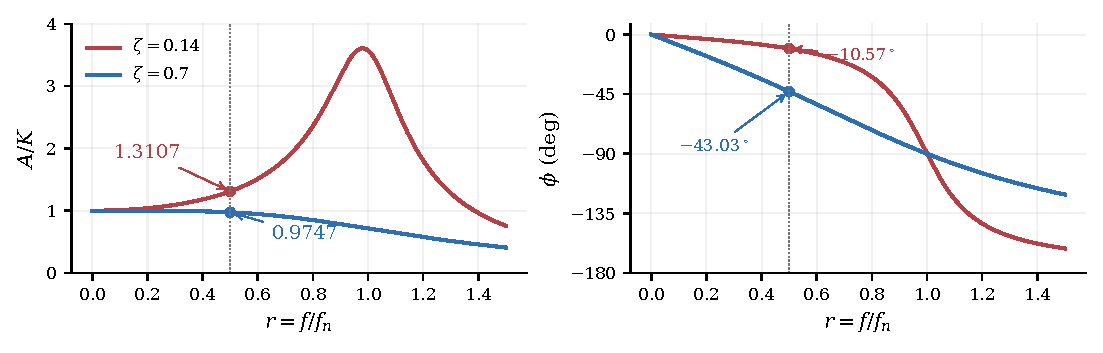
\includegraphics[width=.96\linewidth]{ch3-hw04-damping.pdf}
\end{center}
图中标出的 $r=0.5$ 即本题工作点。$\zeta=0.14$ 的共振峰在 $r_r\approx0.9802$，峰高约 $3.607$；$\zeta=0.7$ 的峰高仅约 $1.0002$。提高阻尼明显压低共振放大，并使本题工作点的幅值更接近静态标定值；相位滞后却由约 $10.57^\circ$ 增大到约 $43.03^\circ$。这说明适度阻尼改善幅值和瞬态振铃，同时需要接受并检查相位延迟。

\begin{focusbox}{知识主线}
把输入频率换成归一化工作点 $r=f/f_n$，由幅相响应评价该点的误差。静态标定、动态幅值校正和时延评价回答不同的问题；选择固有频率时应检查整个待测频带，不能只检查是否低于固有频率。
\end{focusbox}

\subsection*{本题知识点与公式}
\label{kn:3-4}
\noindent\textbf{已学前置：}第\ref{kn:3-3}节的二阶模型、频率比、幅相响应和阻尼折中，第\ref{kn:3-2}节的误差约束。
\textbf{本题新增：}工作点与动态灵敏度、静态标定后的动态误差、已知模型的单频校正、固有频率选取、相位延迟与群延迟。

\subsubsection*{1. 频率比如何把具体传感器放到通用曲线上}
二阶归一化特性只依赖 $r$ 和 $\zeta$，而非分别依赖输入频率与固有频率。因此同一阻尼下，把横轴写成 $r=f/f_n$，不同固有频率装置都可在同一条曲线上比较。这里 $f$ 与 $f_n$ 必须同用Hz，或 $\omega$ 与 $\omega_n$ 同用 $\mathrm{rad/s}$；不能一个用Hz、另一个用角频率。本题 $r=0.5$，表示输入角频率是无阻尼固有角频率的一半，不表示“输入已低到可以忽略所有动态误差”。

在此工作点，分母实部 $1-r^2=0.75$ 固定，虚部 $2\zeta r=\zeta$ 随阻尼变化。所以增大 $\zeta$ 会增大分母的模，使 $A$ 从 $1.310694$ 降到 $0.974740$；同时分母相角增大，使相位更滞后。由复平面上同一个分母即可解释幅值改善、相位滞后增大同时发生的原因。

\subsubsection*{2. 静态灵敏度、动态灵敏度与幅值校正}
设力传感器实际输出电压为 $U$，静态灵敏度为 $K_0>0$，单位 $\mathrm{V/N}$。若采用本题的二阶模型，其实际频率响应为
\[
H_{UF}(\iu\omega)=\frac{K_0}{1-r^2+\iu2\zeta r},\qquad
S_{\mathrm{dyn}}(\omega)=|H_{UF}(\iu\omega)|=K_0A(r).
\]
$S_{\mathrm{dyn}}$ 称该频率下的幅值动态灵敏度，单位仍是 $\mathrm{V/N}$；$A(r)$ 才是无量纲比值。静态标定把电压换为指示力 $z=U/K_0$，所以单频输入力幅值为 $F_0$ 时，指示幅值为 $Z_0=A(r)F_0$。有符号动态偏差为 $(A-1)\times100\%$，误差大小为 $|A-1|\times100\%$。

因此静态标定已知，并没有消除频率相关误差：本题两种阻尼分别仍会高估31.0694\%和低估2.5260\%。若频率和模型参数已准确获知，可按
\[
F_0=\frac{U_0}{K_0A(r)},\qquad
\theta_F=\theta_U-\phi(r)
\]
对单频的幅值与相位作动态校正，其中 $U_0,\theta_U$ 是所测输出电压的幅值和相位。复数形式就是 $\widehat F=\widehat U/H_{UF}(\iu\omega)$。多频信号必须逐频校正，不能用一个常数修正所有频率。

校正的适用前提是装置在线性范围内，$K_0,f_n,\zeta$ 及测量频率已知，而且该频率的输出具有足够信噪比。若输出中有噪声，其折算到输入的幅值会被 $1/|H_{UF}|$ 放大；当高频响应很小时，逆校正会明显放大噪声与模型误差。动态校正因而不能替代合理的传感器带宽与固有频率设计。

\subsubsection*{3. 如何按误差要求选择固有频率}
提高 $f_n$ 会减小给定 $f$ 的 $r$，使工作点靠近 $A(0)=1$、$\phi(0)=0$。但需要多高的 $f_n$，应由误差限和阻尼共同决定，不能仅要求 $f_n>f$。

设待测最高频率为 $f_m$，允许归一化幅值误差为 $0<\varepsilon<1$。从 $|A(r)-1|\leq\varepsilon$ 得
\[
1-\varepsilon\leq A(r)\leq1+\varepsilon.
\]
用第\ref{kn:3-3}节的 $D(r)=A^{-2}(r)$ 代入，等价于
\[
\boxed{\frac{1}{(1+\varepsilon)^2}
\leq1+(4\zeta^2-2)r^2+r^4
\leq\frac{1}{(1-\varepsilon)^2}}.
\]
给定 $\zeta$ 后，这是一组关于 $r$ 的不等式；令 $u=r^2\geq0$，即可化为二次不等式求解。应选出\textbf{从直流 $r=0$ 连续延伸且全段满足要求}的工作区间 $[0,r_A]$，再要求 $f_m/f_n\leq r_A$。低阻尼幅值先升后降，某个较高频率处偶然再次接近1，并不能证明此前整个频带都满足精度。

若还要求 $|\phi|\leq\phi_{\max}<\pi/2$，工作点必须位于 $r<1$。由
$2\zeta r/(1-r^2)\leq\tan\phi_{\max}$，整理二次不等式可得
\[
r\leq r_\phi
=\frac{\sqrt{\zeta^2+\tan^2\phi_{\max}}-\zeta}
{\tan\phi_{\max}},\qquad \phi_{\max}>0.
\]
所以覆盖从直流到 $f_m$ 的设计条件为
\[
\boxed{f_n\geq\frac{f_m}{\min(r_A,r_\phi)}}.
\]
这里的误差限是一般设计符号，原题并未指定，故无需为本题另造数值要求。原题给定 $f_n=800\,\mathrm{Hz}$ 后，直接在 $r=0.5$ 处检查即可；两种阻尼的误差比较已说明它们不能仅凭相同的固有频率视作等效装置。

\subsubsection*{4. 相位差换算的延迟与群延迟不是同一量}
对某个单频输入，若输出滞后 $\phi(\omega)$，可把它写成 $\omega(t-t_\phi)$，定义相位延迟
\[
\boxed{t_\phi(\omega)=-\frac{\phi(\omega)}{\omega}}.
\]
相位须用弧度，结果才是秒；应使用从低频连续展开的相位支。单频的周期性使延迟还存在整周期的不确定性，连续支约定用于在频率之间一致比较。本题输入角频率为 $800\pi\,\mathrm{rad/s}$，两种阻尼的相位延迟约为 $0.07343$ 与 $0.29879\,\mathrm{ms}$。该数值只表示此单频分量的相移，不能直接当作任何波形的整体传播时间。

若信号由某中心角频率 $\omega_c$ 附近的一小段频带组成，可在该处展开相位：
\[
\phi(\omega)\approx\phi(\omega_c)
+\left.\frac{\diff\phi}{\diff\omega}\right|_{\omega_c}(\omega-\omega_c).
\]
当该小频带内幅值近似不变、相位可近似成这条直线时，缓变包络经历的延迟由相位曲线的斜率决定，定义为\textbf{群延迟}
\[
\boxed{t_g(\omega)=-\frac{\diff\phi}{\diff\omega}}.
\]
相位延迟是相位与频率之比，群延迟是相位对频率的导数，单位均为秒。只有纯延迟 $\phi=-\omega t_d$ 时二者都等于同一个 $t_d$；频率相关相位一般不会使二者相等。

例如，一阶装置由第\ref{kn:3-1}节相位式直接得到
\[
t_\phi=\frac{\arctan(\omega\tau)}{\omega},\qquad
t_g=\frac{\tau}{1+(\omega\tau)^2}.
\]
二阶装置对 $\operatorname{atan2}(2\zeta r,1-r^2)$ 求导，分子为
$(1-r^2)2\zeta-(2\zeta r)(-2r)=2\zeta(1+r^2)$，再用 $\diff r/\diff\omega=1/\omega_n$，得到
\[
t_g(\omega)=\frac{2\zeta(1+r^2)}
{\omega_n\bigl[(1-r^2)^2+4\zeta^2r^2\bigr]}.
\]
在本题 $r=0.5$ 处，两种阻尼的群延迟约为 $0.11962$ 与 $0.33079\,\mathrm{ms}$，均与各自相位延迟不同。在 $r\to0$ 的极限下，两者才都趋向 $2\zeta/\omega_n$，与上一题的近似线性相位相符。理解这一差别，就能区分“某频率相位滞后较大”和“某个多频波形是否近似共同延迟”这两个判断。
\nt{\textbf{易错点：}本题 $r=0.5$ 并非共振点；“幅值比更接近1”不等于“相位滞后更小”。实际电压输出还需乘力传感器的静态灵敏度，题中未给出该值，不能为它指定数值。}
